% The RHM and the tree tensor network, 2026-11-18: an expansion of the first four slides of ../2026-11-18-rhm
% (the grammar, the architectures, sample complexity, the architecture controls, and what the bonds hold).
% No hidden-Markov or toy-grammar material; that is in the other deck.
% Build from this directory with: latexmk -pdf -halt-on-error slides.tex
% What to say on each slide is in script.md.
% Figures: figures/make_figures.py redraws them from the saved results (run from the repository root).
% Tensor network diagrams use tensor-network.sty from github.com/mptoolkit/tikz-diagrams (GPL-3), copied here.
\documentclass[aspectratio=169,12pt,t]{beamer}
\usepackage[T1]{fontenc}
\usepackage{lmodern,tgpagella,tgheros}
\usepackage{amsmath,amssymb,graphicx,tikz,booktabs,array}
\usepackage{tensor-network}
\usepackage{pifont}
\newcommand{\yes}{\ding{51}}
\newcommand{\no}{\ding{55}}
\usetikzlibrary{arrows.meta,calc}
\usefonttheme[onlymath]{serif}
\definecolor{ink}{gray}{0.09}
\definecolor{secondary}{gray}{0.33}
\definecolor{aligned}{HTML}{0F4D92}   % figures4papers blue: the tree that matches the grammar
\definecolor{crossed}{HTML}{B64342}   % figures4papers red: the tree that does not
\definecolor{f4teal}{HTML}{42949E}
\definecolor{f4violet}{HTML}{9A4D8E}
\setbeamercolor{normal text}{fg=ink,bg=white}
\setbeamercolor{structure}{fg=ink}
\setbeamercolor{frametitle}{fg=ink,bg=white}
\setbeamerfont{title}{family=\rmfamily,series=\bfseries}
\setbeamerfont{frametitle}{parent=title,size=\Large}
\setbeamerfont{block title}{family=\rmfamily,series=\bfseries}
\setbeamersize{text margin left=9mm,text margin right=9mm}
\setbeamertemplate{navigation symbols}{}
\setbeamertemplate{headline}{}
\setbeamertemplate{footline}{}
\setbeamertemplate{frametitle}{%
  \vspace*{4mm}\noindent\usebeamerfont{frametitle}\insertframetitle\par}
\setbeamertemplate{itemize item}{\raisebox{0.2ex}{\tiny$\bullet$}}
\setbeamertemplate{enumerate item}{\insertenumlabel.}
\newcommand{\contextline}[1]{{\par\centering\small\color{secondary}#1\par}}
\newcommand{\sym}{\textsf{sym}}
\newcommand{\modg}{\textsf{mod}}
\newcommand{\rd}{\mathrm{read}}
\hypersetup{pdftitle={Tree tensor networks on the Random Hierarchy Model},pdfauthor={}}

% Tensor network pictures: circles are trained cores, dots are data, every edge carries its dimension.
\tnsetup{tensorsize=11pt, xscale=1, yscale=1, outer xsep=0pt, outer ysep=0pt, tensor fill=gray!12}
\tikzset{
  dim/.style={font=\scriptsize, inner sep=1.2pt, text=ink},
  data/.style={circle, fill=ink, inner sep=0pt, minimum size=3.2pt},
  lev/.style={anchor=west, font=\footnotesize, align=left, text=ink, inner sep=0pt},
  levsec/.style={lev, text=secondary}}

\begin{document}

% ---------------------------------------------------------------------------------------------------------------
% The grammar. Source: studies/rhm/grammar.py. Standard configuration v = n = 16, m = 4, s = 2, L = 4.
\begin{frame}{The Random Hierarchy Model}
  \vspace{3mm}
  \begin{columns}[c,onlytextwidth]
    \begin{column}{.60\linewidth}
      \centering
      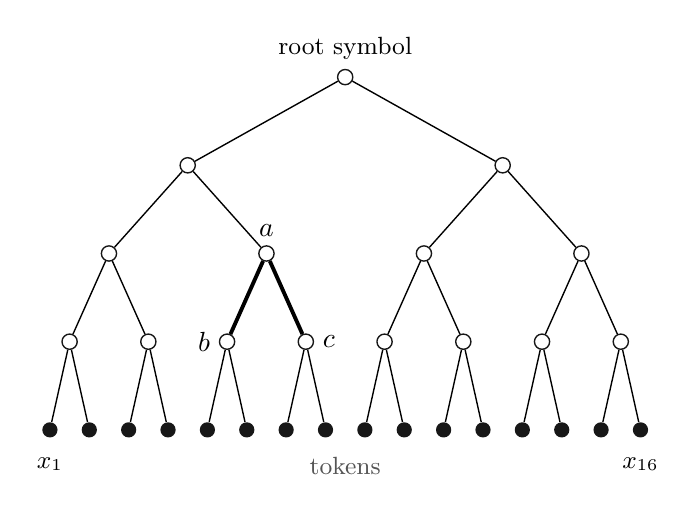
\begin{tikzpicture}[x=0.5cm,y=1.12cm,
          latent/.style={circle,draw=ink,fill=white,inner sep=0pt,minimum size=5.5pt,line width=.5pt},
          token/.style={circle,fill=ink,inner sep=0pt,minimum size=5.5pt}]
        % level l has 2^l nodes; node k of level l sits above the middle of its 2^(4-l) tokens
        \foreach \l/\cnt/\wid in {0/1/16,1/2/8,2/4/4,3/8/2}{
          \foreach \k in {1,...,\cnt}{
            \pgfmathsetmacro{\x}{(\k-0.5)*\wid-0.5}
            \node[latent] (n\l-\k) at (\x,4-\l) {};
          }
        }
        \foreach \k in {1,...,16}{ \node[token] (n4-\k) at (\k-1,0) {}; }
        \foreach \l/\cnt in {0/1,1/2,2/4,3/8}{
          \pgfmathtruncatemacro{\next}{\l+1}
          \foreach \k in {1,...,\cnt}{
            \pgfmathtruncatemacro{\a}{2*\k-1}
            \pgfmathtruncatemacro{\b}{2*\k}
            \draw[line width=.5pt] (n\l-\k) -- (n\next-\a);
            \draw[line width=.5pt] (n\l-\k) -- (n\next-\b);
          }
        }
        % one production, drawn heavier
        \draw[line width=1.4pt] (n2-2) -- (n3-3) (n2-2) -- (n3-4);
        \node[anchor=south,inner sep=3pt] at (n2-2.north) {$a$};
        \node[anchor=east,inner sep=3pt] at (n3-3.west) {$b$};
        \node[anchor=west,inner sep=3pt] at (n3-4.east) {$c$};
        \node[font=\small,anchor=south] at (n0-1.north) {root symbol};
        \node[font=\small,anchor=north] at (0,-0.2) {$x_1$};
        \node[font=\small,anchor=north] at (15,-0.2) {$x_{16}$};
        \node[font=\small,anchor=north,text=secondary] at (7.5,-0.2) {tokens};
      \end{tikzpicture}
    \end{column}
    \begin{column}{.38\linewidth}
      \[ a \;\to\; b\,c \mid d\,e \mid f\,g \mid h\,k \]
      \contextline{$m=4$ synonyms per symbol}
      \vspace{5mm}
      \[
        \begin{aligned}
          \textbf{root:}\quad & x_{1:16} \mapsto \text{root symbol}\\
          \textbf{last:}\quad & x_{1:15} \mapsto x_{16}
        \end{aligned}
      \]
      \vspace{1mm}
      \[ P^* = n\,m^L = 4{,}096 \]
    \end{column}
  \end{columns}
  \vspace{3mm}
  \contextline{$v = n = 16$ symbols per level, depth $L=4$ \qquad Cagnetta et al.\ (2024)}
\end{frame}

% ---------------------------------------------------------------------------------------------------------------
% The model. Source: ctn/tree.py (TreeTN). Parameters n V r + (n - 2) r^3 + O r^2 = 65,536 at V = r = O = 16:
% 16 x 256 (embeddings) + 14 x 4,096 (fusion cores) + 4,096 (root core).
\begin{frame}{The tree tensor network has the grammar's shape}
  \vspace{3mm}
  \centering
  \begin{tikzpicture}[tensornetwork, x=0.54cm, y=0.94cm, line width=0.5pt]
    % leaves: data dot, physical leg of dimension V, embedding A_i
    \foreach \k in {1,...,16}{
      \node[data] (x\k) at (\k-1,0) {};
      \node[atensor] (t0-\k) at (\k-1,0.85) {};
      \draw (x\k) -- (t0-\k) node[dim,midway,right] {$V$};
    }
    % fusion cores, level l = 1..3, then the root core
    \foreach \l/\cnt/\wid in {1/8/2,2/4/4,3/2/8}{
      \foreach \k in {1,...,\cnt}{
        \pgfmathsetmacro{\x}{(\k-0.5)*\wid-0.5}
        \node[atensor] (t\l-\k) at (\x,0.85+\l) {};
      }
    }
    \node[atensor] (C) at (7.5,4.85) {};
    \foreach \l/\cnt in {1/8,2/4,3/2}{
      \pgfmathtruncatemacro{\prev}{\l-1}
      \foreach \k in {1,...,\cnt}{
        \pgfmathtruncatemacro{\a}{2*\k-1}
        \pgfmathtruncatemacro{\b}{2*\k}
        \draw (t\prev-\a) -- (t\l-\k) node[dim,midway,left] {$r$};
        \draw (t\prev-\b) -- (t\l-\k) node[dim,midway,right] {$r$};
      }
    }
    \draw (t3-1) -- (C) node[dim,midway,above left] {$r$};
    \draw (t3-2) -- (C) node[dim,midway,above right] {$r$};
    \draw (C) -- ++(0,0.7) node[dim,midway,right] {$O$} coordinate (out);
    \node[font=\footnotesize,anchor=south,inner sep=2pt] at (out) {logits, $O=16$};
    \node[font=\footnotesize,anchor=north] at (0,-0.15) {$x_1$};
    \node[font=\footnotesize,anchor=north] at (15,-0.15) {$x_{16}$};
    % each level: its tensors, their shape, and the parameter count at V = r = O = 16
    \def\xl{16.6}
    \def\xp{25.6}
    \node[lev] at (\xl,4.85) {$C\in\mathbb{R}^{O\times r\times r}$};
    \node[lev] at (\xl,3.85) {$2\times W\in\mathbb{R}^{r\times r\times r}$};
    \node[lev] at (\xl,2.85) {$4\times W$};
    \node[lev] at (\xl,1.85) {$8\times W$};
    \node[lev] at (\xl,0.85) {$16\times A_i\in\mathbb{R}^{r\times V}$};
    \node[lev] at (\xl,0) {one-hot, $V=16$};
    \foreach \y/\n in {4.85/{4{,}096},3.85/{8{,}192},2.85/{16{,}384},1.85/{32{,}768},0.85/{4{,}096}}{
      \node[levsec,anchor=east] at (\xp,\y) {\n};
    }
    \draw[secondary,line width=0.4pt] (\xp-2.6,0.4) -- (\xp,0.4);
    \node[levsec,anchor=east] at (\xp,0) {65{,}536};
    \node[levsec,anchor=east] at (\xp,5.45) {parameters, $r=16$};
  \end{tikzpicture}

  \vspace{4mm}
  \(z_i = A_i\,e_{x_i}, \qquad
    z_{\text{parent}} = W(z_{\text{left}}, z_{\text{right}}), \qquad
    \text{logits} = C(z_{\mathrm L}, z_{\mathrm R})\)
\end{frame}

% ---------------------------------------------------------------------------------------------------------------
% The two tree controls of rhm-controls. Source: ctn/tree.py (TreeTN, tie='level' and perm).
% Tied: 16 x 16 (one A) + 3 x 4,096 (one W per level) + 4,096 (C) = 16,640. The permutation drawn is the one of
% grammar 0, init seed 0 (rhm-controls/results/analysis.json, meta.perms.g0_s0): leaf i reads token perm[i].
\begin{frame}{Two controls change one thing in the tree}
  \vspace{1mm}
  \centering
  \begin{tikzpicture}[tensornetwork, x=0.37cm, y=0.8cm, line width=0.5pt,
      dim/.append style={font=\tiny, inner sep=0.8pt}]
    % ---------------- tied tree: one fill per shared tensor ----------------
    \begin{scope}
      \foreach \k in {1,...,16}{
        \node[data] (x\k) at (\k-1,0) {};
        \node[atensor, fill=gray!25] (t0-\k) at (\k-1,0.85) {};
        \draw (x\k) -- (t0-\k) node[dim,midway,right] {$V$};
      }
      \foreach \l/\cnt/\wid/\col in {1/8/2/f4teal!40,2/4/4/aligned!35,3/2/8/f4violet!40}{
        \foreach \k in {1,...,\cnt}{
          \pgfmathsetmacro{\x}{(\k-0.5)*\wid-0.5}
          \node[atensor, fill=\col] (t\l-\k) at (\x,0.85+\l) {};
        }
      }
      \node[atensor, fill=white] (C) at (7.5,4.85) {};
      \foreach \l/\cnt in {1/8,2/4,3/2}{
        \pgfmathtruncatemacro{\prev}{\l-1}
        \foreach \k in {1,...,\cnt}{
          \pgfmathtruncatemacro{\a}{2*\k-1}
          \pgfmathtruncatemacro{\b}{2*\k}
          \draw (t\prev-\a) -- (t\l-\k) node[dim,midway,left] {$r$};
          \draw (t\prev-\b) -- (t\l-\k) node[dim,midway,right] {$r$};
        }
      }
      \draw (t3-1) -- (C) node[dim,midway,above left] {$r$};
      \draw (t3-2) -- (C) node[dim,midway,above right] {$r$};
      \draw (C) -- ++(0,0.6) node[dim,midway,right] {$O$};
      \foreach \y/\t in {4.85/$C$,3.85/$W_3$,2.85/$W_2$,1.85/$W_1$,0.85/$A$}{
        \node[font=\footnotesize,anchor=east] at (-1.3,\y) {\t};
      }
      \node[font=\footnotesize,anchor=north] at (0,-0.15) {$x_1$};
      \node[font=\footnotesize,anchor=north] at (15,-0.15) {$x_{16}$};
      \node[font=\small,anchor=north,align=center] at (7.5,-0.95)
        {\textbf{tied}: one $A$, one $W$ per level\\ {\color{secondary}16{,}640 parameters}};
    \end{scope}
    % ---------------- permuted tree: the same cores, leaves read permuted tokens ----------------
    \begin{scope}[xshift=7.25cm]
      \foreach \k in {1,...,16}{
        \node[data] (x\k) at (\k-1,-0.55) {};
        \node[atensor] (t0-\k) at (\k-1,0.85) {};
        \coordinate (s\k) at (\k-1,0.42);
        \draw (t0-\k) -- (s\k) node[dim,midway,right] {$V$};
      }
      % leaf i (1-based) reads token perm[i-1] + 1, perm = [10,4,7,3,6,8,11,1,15,13,9,0,2,12,5,14]
      \foreach \leaf/\tok in {1/11,2/5,3/8,4/4,5/7,6/9,7/12,8/2,9/16,10/14,11/10,12/1,13/3,14/13,15/6,16/15}{
        \draw[crossed, line width=0.45pt] (s\leaf) -- (x\tok);
      }
      \foreach \l/\cnt/\wid in {1/8/2,2/4/4,3/2/8}{
        \foreach \k in {1,...,\cnt}{
          \pgfmathsetmacro{\x}{(\k-0.5)*\wid-0.5}
          \node[atensor] (t\l-\k) at (\x,0.85+\l) {};
        }
      }
      \node[atensor] (C) at (7.5,4.85) {};
      \foreach \l/\cnt in {1/8,2/4,3/2}{
        \pgfmathtruncatemacro{\prev}{\l-1}
        \foreach \k in {1,...,\cnt}{
          \pgfmathtruncatemacro{\a}{2*\k-1}
          \pgfmathtruncatemacro{\b}{2*\k}
          \draw (t\prev-\a) -- (t\l-\k) node[dim,midway,left] {$r$};
          \draw (t\prev-\b) -- (t\l-\k) node[dim,midway,right] {$r$};
        }
      }
      \draw (t3-1) -- (C) node[dim,midway,above left] {$r$};
      \draw (t3-2) -- (C) node[dim,midway,above right] {$r$};
      \draw (C) -- ++(0,0.6) node[dim,midway,right] {$O$};
      \node[font=\footnotesize,anchor=north] at (0,-0.7) {$x_1$};
      \node[font=\footnotesize,anchor=north] at (15,-0.7) {$x_{16}$};
      \node[font=\small,anchor=north,align=center] at (7.5,-0.95)
        {\textbf{permuted}: leaf $i$ reads $x_{\pi(i)}$\\ {\color{secondary}65{,}536 parameters}};
    \end{scope}
  \end{tikzpicture}

  \vspace{1mm}
  \contextline{$V = r = O = 16$ in both \qquad same fill $=$ one shared tensor}
\end{frame}

% ---------------------------------------------------------------------------------------------------------------
% The chain of rhm-controls. Source: ctn/tree.py (ChainTN): h_0 learned, h_t = W(h_{t-1}, A e_{x_t}), logits = U h_16.
% Parameters r + V r + r^3 + O r = 40 + 640 + 64,000 + 640 = 65,320 at r = 40, V = O = 16.
\begin{frame}{The chain matches the tree's parameter count}
  \vspace{6mm}
  \centering
  \begin{tikzpicture}[tensornetwork, x=0.78cm, y=1.0cm, line width=0.5pt]
    \node[atensor, fill=white] (h0) at (0,0) {};
    \node[font=\footnotesize,anchor=south,inner sep=3pt] at (h0.north) {$h_0$};
    \foreach \k in {1,...,16}{
      \node[atensor, fill=f4violet!40] (w\k) at (\k,0) {};
      \node[atensor, fill=gray!25] (a\k) at (\k,-1) {};
      \node[data] (x\k) at (\k,-1.85) {};
      \draw (w\k) -- (a\k) node[dim,midway,right] {40};
      \draw (a\k) -- (x\k) node[dim,midway,right] {16};
    }
    \draw (h0) -- (w1) node[dim,midway,anchor=south,yshift=2.5pt] {40};
    \foreach \k in {1,...,15}{
      \pgfmathtruncatemacro{\n}{\k+1}
      \draw (w\k) -- (w\n) node[dim,midway,anchor=south,yshift=2.5pt] {40};
    }
    \node[atensor, fill=white] (U) at (17,0) {};
    \node[font=\footnotesize,anchor=south,inner sep=3pt] at (U.north) {$U$};
    \draw (w16) -- (U) node[dim,midway,anchor=south,yshift=2.5pt] {40};
    \draw (U) -- ++(0,-0.8) node[dim,midway,right] {16} coordinate (out);
    \node[font=\footnotesize,anchor=north,inner sep=2pt] at (out) {logits};
    \node[font=\footnotesize,anchor=south,inner sep=3pt] at ([yshift=4pt]w1.north) {$W$};
    \node[font=\footnotesize,anchor=east] at (0.55,-1) {$A$};
    \node[font=\footnotesize,anchor=north] at (1,-2.0) {$x_1$};
    \node[font=\footnotesize,anchor=north] at (16,-2.0) {$x_{16}$};
  \end{tikzpicture}

  \vspace{6mm}
  \(h_t = W\big(h_{t-1},\, A\,e_{x_t}\big), \qquad \text{logits} = U\,h_{16}\)

  \vspace{5mm}
  {\small\(h_0\!: 40 \qquad\quad A\in\mathbb{R}^{40\times16}\!: 640 \qquad\quad W\in\mathbb{R}^{40\times40\times40}\!: 64{,}000 \qquad\quad U\in\mathbb{R}^{16\times40}\!: 640\)}

  \vspace{4mm}
  \contextline{65{,}320 parameters (tree: 65{,}536) \qquad one $W$ and one $A$ for all positions}
\end{frame}

% ---------------------------------------------------------------------------------------------------------------
% figures/samples.pdf, from rhm-sample-efficiency/results/analysis.json. Numbers: rhm-sample-efficiency/README.md.
\begin{frame}{The tree learns the root between $P^*$ and $4P^*$}
  \vspace{1mm}
  \centering
  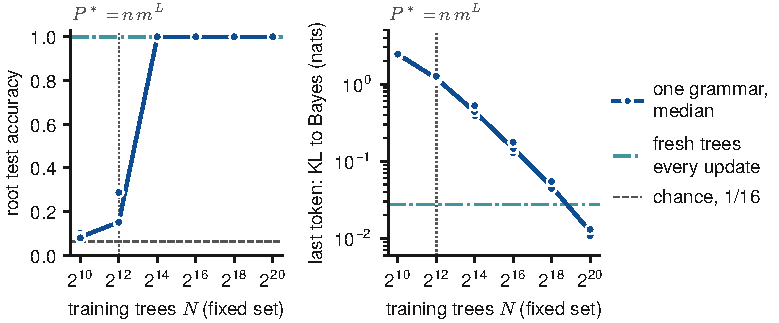
\includegraphics[width=\linewidth,height=.70\paperheight,keepaspectratio]{figures/samples.pdf}\par
  \medskip
  \contextline{untied tree, $r = 16$, three grammars per size \qquad $P^* = 4{,}096$}
\end{frame}

% ---------------------------------------------------------------------------------------------------------------
% figures/memorize.pdf, from rhm-sample-efficiency/results/curves.json (root task, grammar 0).
\begin{frame}{At $N \le P^*$ the tree memorizes its training set}
  \vspace{1mm}
  \centering
  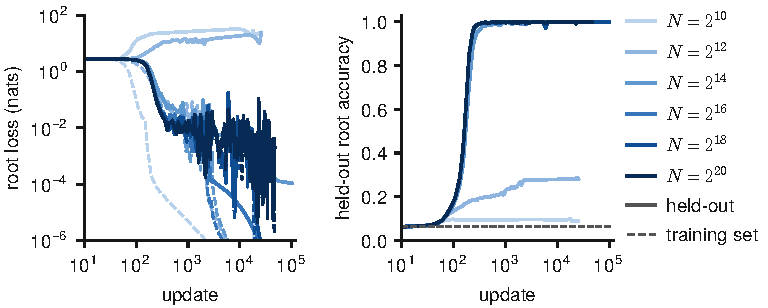
\includegraphics[width=\linewidth,height=.70\paperheight,keepaspectratio]{figures/memorize.pdf}\par
  \medskip
  \contextline{root task, grammar 0 \qquad all 12 runs that fail to learn fit their training set}
\end{frame}

% ---------------------------------------------------------------------------------------------------------------
% figures/arch_curves.pdf, from rhm-controls/results/curves.json. Numbers: rhm-controls/README.md.
\begin{frame}{On fresh data, only the matching trees reach Bayes}
  \vspace{1mm}
  \centering
  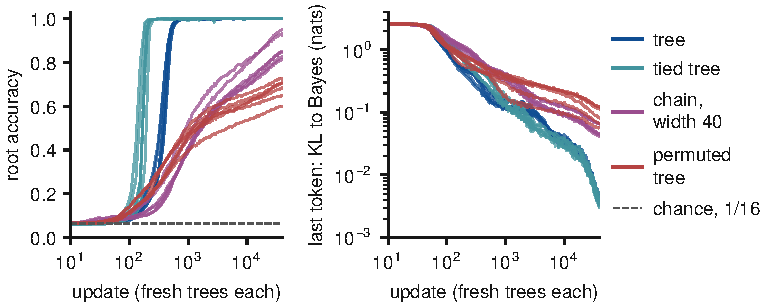
\includegraphics[width=\linewidth,height=.70\paperheight,keepaspectratio]{figures/arch_curves.pdf}\par
  \medskip
  \contextline{six runs per architecture and task: three grammars $\times$ two inits \qquad 40{,}000 updates}
\end{frame}

% ---------------------------------------------------------------------------------------------------------------
% figures/arch_final.pdf, from rhm-controls/results/curves.json; the medians agree with the table in rhm-controls/README.md.
\begin{frame}{Tying is free; permuting costs more than a chain}
  \vspace{1mm}
  \centering
  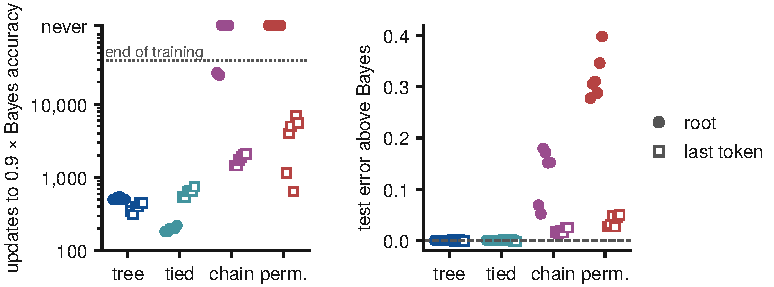
\includegraphics[width=\linewidth,height=.70\paperheight,keepaspectratio]{figures/arch_final.pdf}\par
  \medskip
  \contextline{tree beats permuted, and tied beats chain, in 12 of 12 pairs on both measures}
\end{frame}

% ---------------------------------------------------------------------------------------------------------------
% Numbers: rhm-transfer/README.md, rhm-ttn-belief-geometry/README.md, rhm-ttn-messages/README.md (H1, H2, H4),
% rhm-ttn-masks/README.md. A cell is one grammar at one width with three seeds.
\begin{frame}{What the bonds hold: six tests}
  \vspace{5mm}
  \centering
  \renewcommand{\arraystretch}{1.55}
  \begin{tabular}{@{}cl@{\quad\ }l@{}}
    \yes & lower subtrees transfer & 42 updates frozen, 148 from scratch\\
    \yes & top bonds $\Rightarrow$ Bayes belief & 7 of 8 grammars, $R^2$ 0.85 to 1.00\\
    \yes & bond keeps what the task needs & 7 of 9 cells, 0.81 to 0.96 of variance\\
    \no & bond $=$ the grammar's message & 0 of 9 cells, $R^2$ 0.08 to 0.75\\
    \no & merge $=$ the message update & 0 of 9 cells, $R^2$ 0.17 to 0.58\\
    \no & mixed-mask training repairs it & 0 of 12 runs\\
  \end{tabular}

  \vspace{5mm}
  \contextline{a probe test passes at $R^2 \ge 0.8$ in all three seeds of a cell}
\end{frame}

% ---------------------------------------------------------------------------------------------------------------
% figures/transfer.pdf, from rhm-transfer/results/{curves,analysis}.json. Numbers: rhm-transfer/README.md.
\begin{frame}{Pretrained subtrees transfer to unseen productions}
  \vspace{1mm}
  \centering
  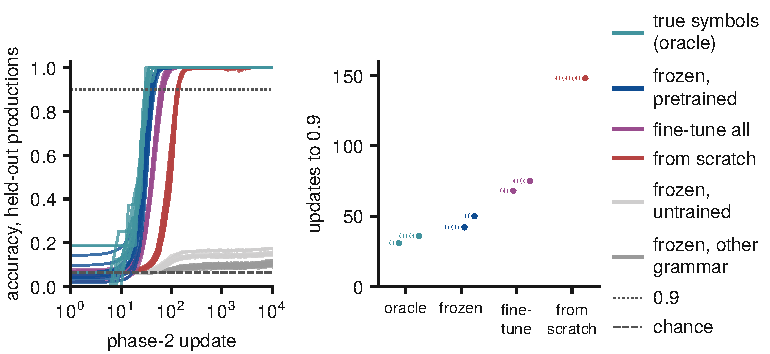
\includegraphics[width=\linewidth,height=.70\paperheight,keepaspectratio]{figures/transfer.pdf}\par
  \medskip
  \contextline{48 root productions in pretraining, 16 held out \qquad nine units per arm}
\end{frame}

% ---------------------------------------------------------------------------------------------------------------
% figures/belief_second.pdf, from rhm-ttn-belief-geometry/results/summary.json (h2_bil, h2_init_bil, h2_addceil, h2_scr).
\begin{frame}{The product of the top bonds gives the belief}
  \vspace{1mm}
  \centering
  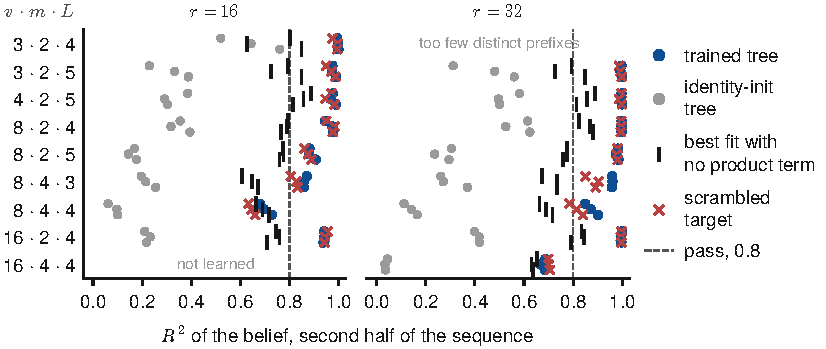
\includegraphics[width=\linewidth,height=.68\paperheight,keepaspectratio]{figures/belief_second.pdf}\par
  \medskip
  \contextline{linear probe on $[h_{\mathrm L}, h_{\mathrm R}, h_{\mathrm L}\!\otimes h_{\mathrm R}]$ \qquad 7 of 8 grammars pass at each width}
\end{frame}

% ---------------------------------------------------------------------------------------------------------------
% figures/belief_first.pdf, from rhm-ttn-belief-geometry/results/summary.json (h1_top, h1_init, h1_nexttok, h1_scr).
\begin{frame}{Without the product, only the small alphabets pass}
  \vspace{1mm}
  \centering
  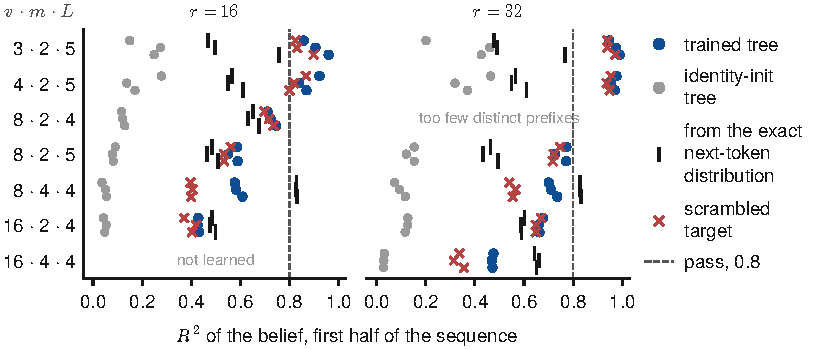
\includegraphics[width=\linewidth,height=.68\paperheight,keepaspectratio]{figures/belief_first.pdf}\par
  \medskip
  \contextline{affine probe on $h_{\mathrm L}$, first half of the sequence \qquad passes in 2 of 6 at each width}
\end{frame}

% ---------------------------------------------------------------------------------------------------------------
% figures/messages.pdf, from rhm-ttn-messages/results/summary.json (m1_proj, m2_ve, m3_acc, m4_both and their controls).
\begin{frame}{Bonds hold what the task needs, not messages}
  \vspace{1mm}
  \centering
  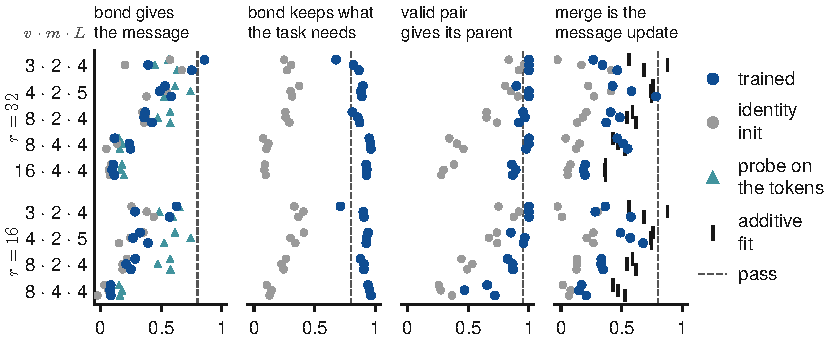
\includegraphics[width=\linewidth,height=.68\paperheight,keepaspectratio]{figures/messages.pdf}\par
  \medskip
  \contextline{nine learned cells, three seeds each \qquad cells passing, left to right: 0, 7, 3, 0 of 9}
\end{frame}

% ---------------------------------------------------------------------------------------------------------------
% figures/masks.pdf, from rhm-ttn-masks/results/summary.json (m4_both, m4_both_ceil, m3_invalid_q). r = 32.
\begin{frame}{Training on mixed masks does not repair the merge}
  \vspace{1mm}
  \centering
  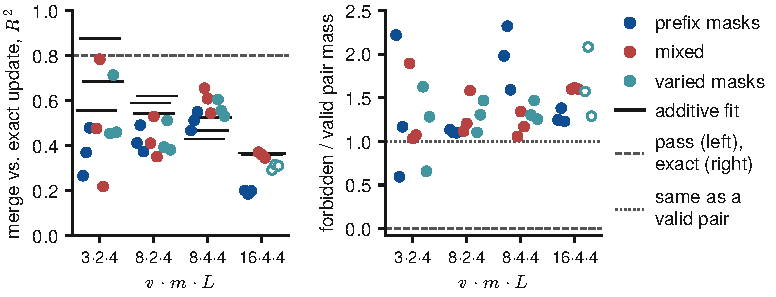
\includegraphics[width=\linewidth,height=.70\paperheight,keepaspectratio]{figures/masks.pdf}\par
  \medskip
  \contextline{$r = 32$ \qquad mixed learned the varied task in only 2 of 4 grammars}
\end{frame}

% ---------------------------------------------------------------------------------------------------------------
% The open checks named in rhm-controls/README.md, rhm-sample-efficiency/README.md and rhm-ttn-masks/README.md.
\begin{frame}{Which check first?}
  \vspace{8mm}
  \begin{enumerate}
    \setlength{\itemsep}{7mm}
    \item A $10^{-2}$ learning-rate pilot for the permuted tree and the chain
    \item Training sets between $2^{12}$ and $2^{14}$, then a sweep over $m$ or $L$
    \item A longer schedule for mixed masks at $m = 4$
  \end{enumerate}
  \vspace{9mm}
  \contextline{each is listed as not yet checked in its experiment's write-up}
\end{frame}

\end{document}
